\section{Endowrist}\label{sec:Endowrist}

An Endowrist, see \figref{fig:Endo_full} is a surgical tool which can be manipulated as a human wrist. It is used in surgical procedures such as Laparoscopic surgeries, better known as minimally invasive surgery (MIS), where small incisions in the human body is made under the surgery. Because the incision cuts are small, blood lose under the surgery and the risk of infection is reduced. This has a positive effect on the recovery time for the patient.


\begin{figure}[H]
	\centering
	\begin{subfigure}{.32\textwidth}
		\centering
		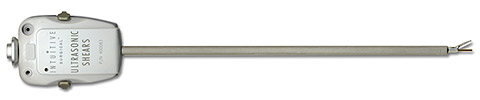
\includegraphics[width=\linewidth]{Endowrist1.jpg}
		\caption{Full view of a Endowrist\vspace{8.5mm}   }
		\label{fig:Endo_full}
	\end{subfigure}
	\begin{subfigure}{.32\textwidth}
		\centering
		\includegraphics[width=\linewidth]{Endowrist2.png}
		\caption{Actuator plates, which can alternate the end effector position}
		\label{fig:Endo_plates}
	\end{subfigure}
	\begin{subfigure}{.32\textwidth}
		\centering
		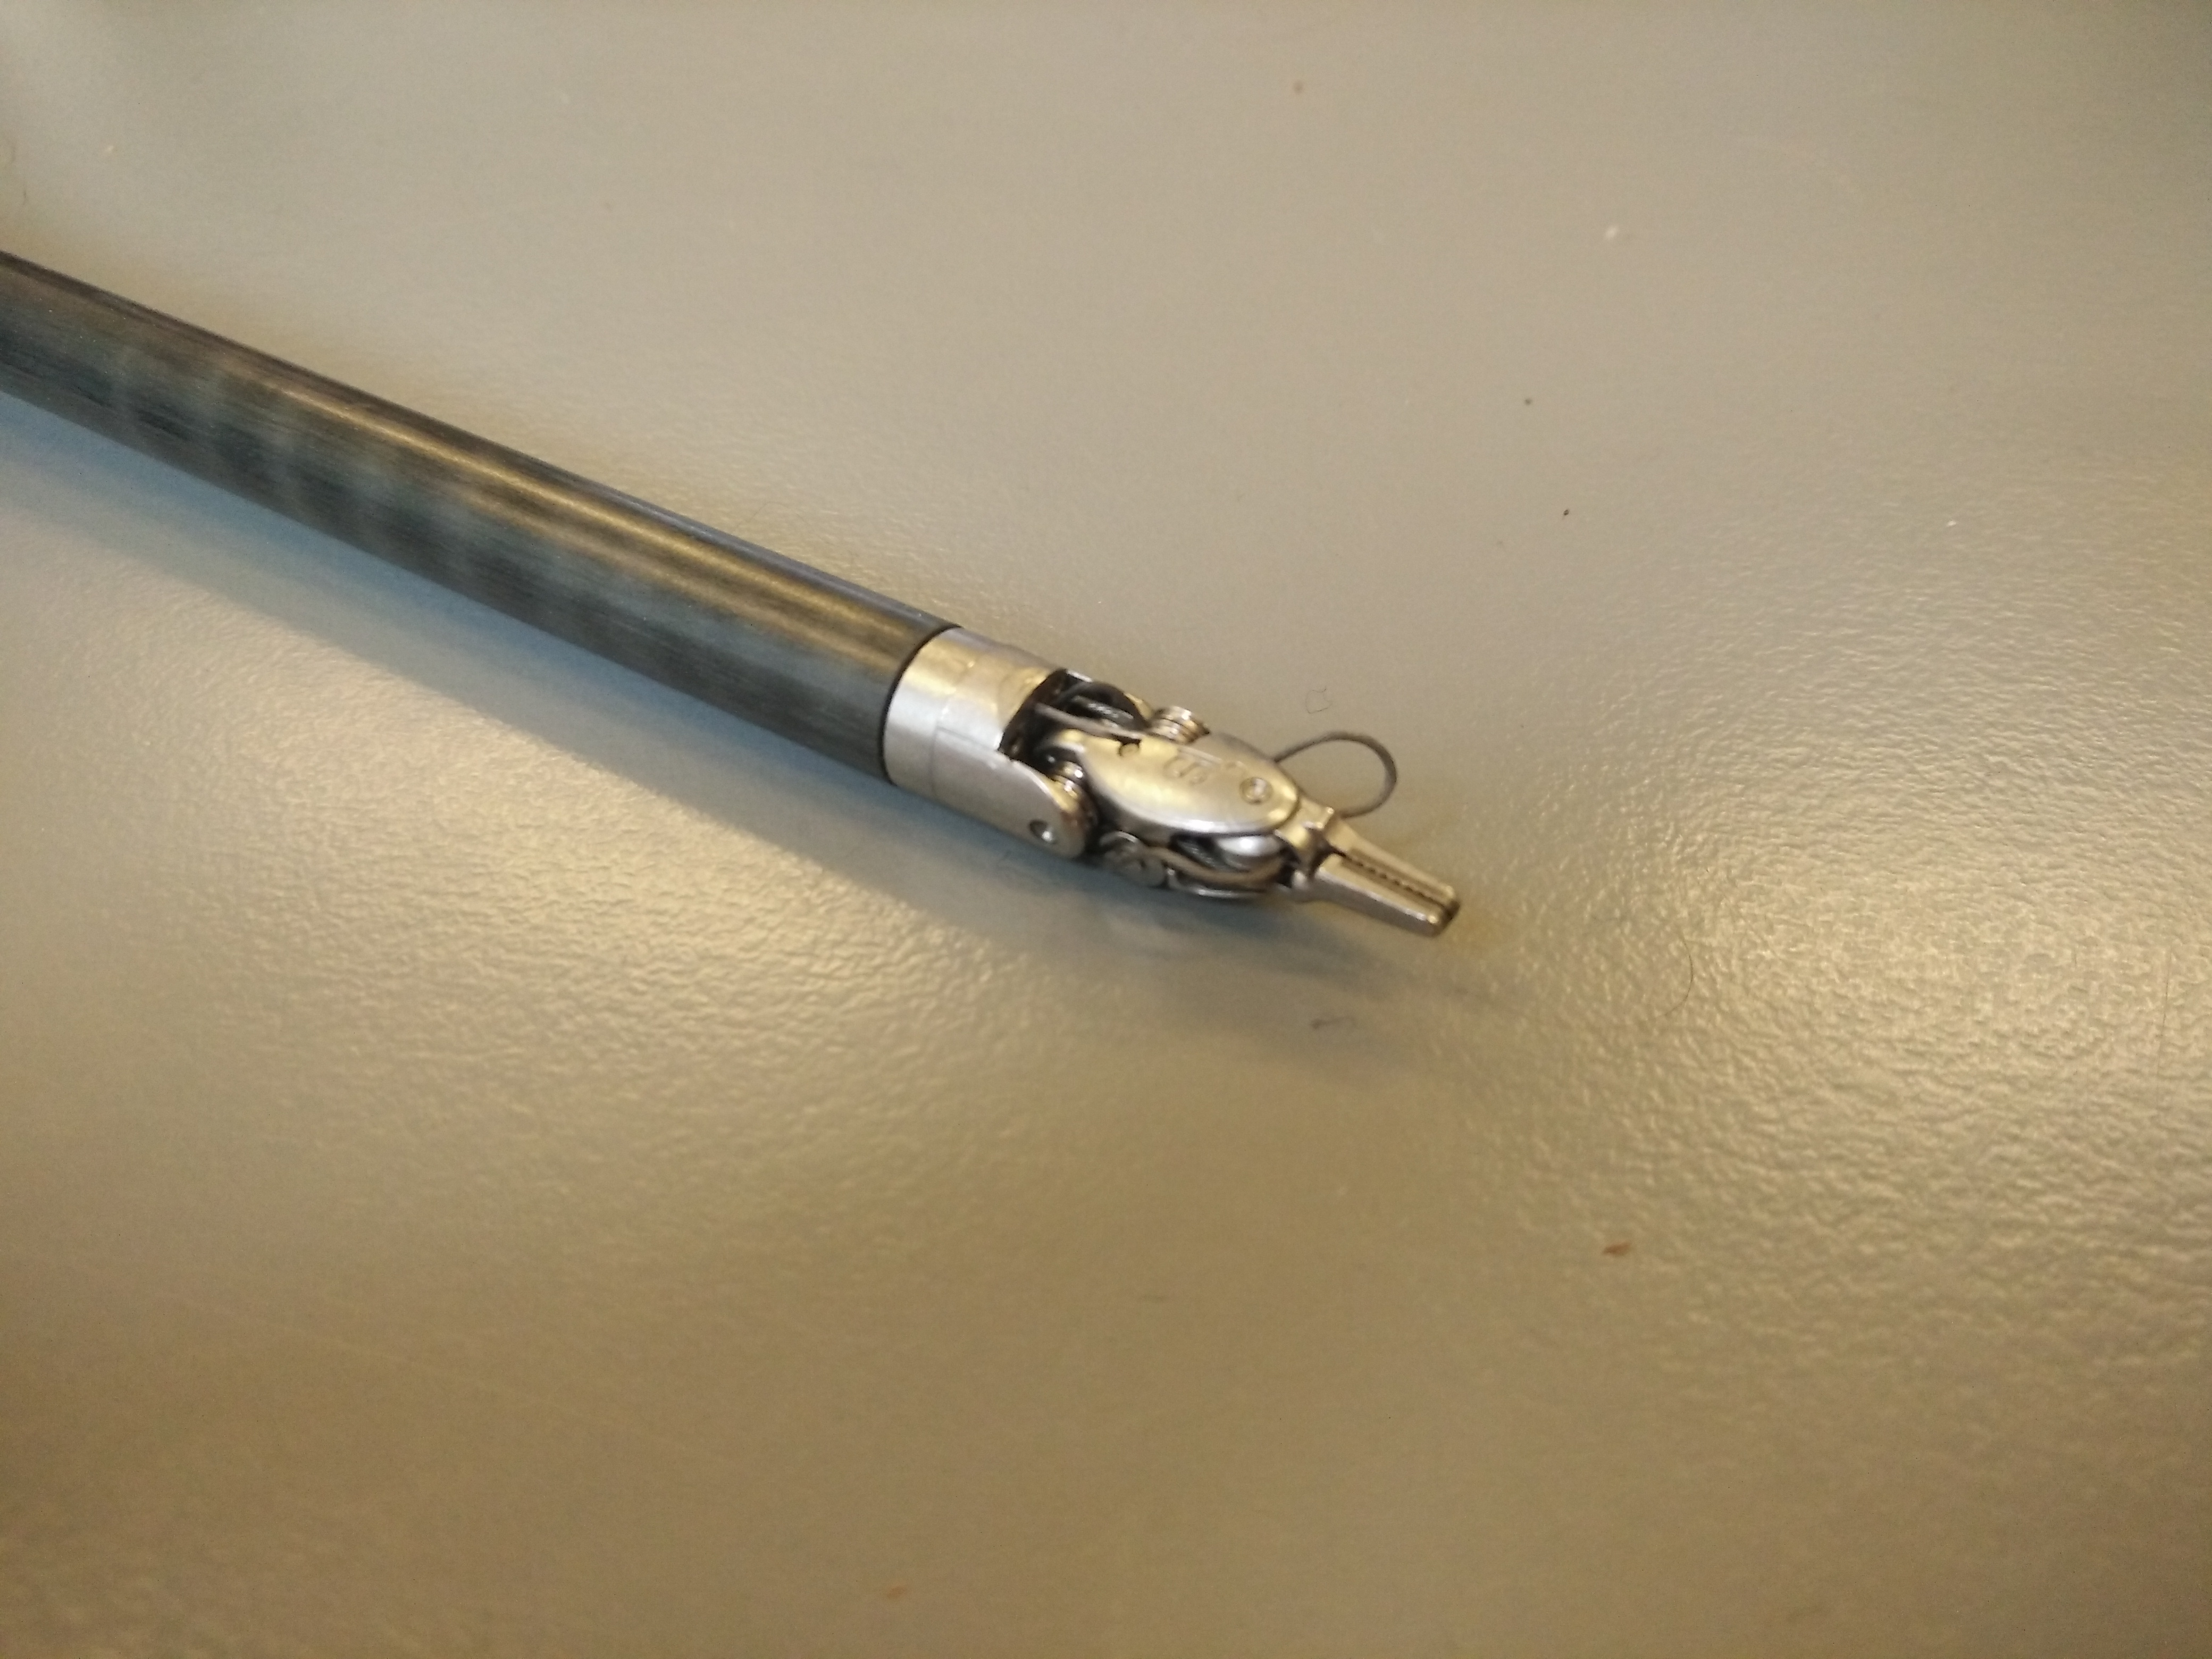
\includegraphics[width=\linewidth]{Endowrist3.jpg}
		\caption{End effector of the Endowrist\newline}
		\label{fig:Endo_end}
	\end{subfigure}
\caption{The Endowrist and how the interaction with it are made}
\label{fig:endowrits_set}
\end{figure}

As mentioned the Endowrist has the ability to be manipulated as a human wrist and thereby has four \gls{DOF}, see \figref{fig:Endo_end}.\todo{We have to update the picture so it shows each DOF}. This enables the movement of roll, pitch, yaw and an open closing mechanism that acts as the thumb and index finger of a hand. 

The end effector is manipulated by the four wheels seen on \figref{fig:Endo_plates}. Wheel one and three define the movement of the yaw and the closing mechanism. Wheel two and four moves the pitch and roll. The Endowrist is cable driven, which enables the opportunity of making the Endowrist small but it also makes the system nonlinear as the force acting at one end is not directly transmitted to the other end due to friction. 



